\section{Results}
\label{sec:results}
We evaluate AXON against the objective in Eq.~\eqref{eq:objective} on the
reference stack (Sec.~\ref{sec:model}) and report: gated-path latency $L$
against the budget $T=100$\,ms (Sec.~\ref{sec:res-latency}); the effect of the
network discipline predicted by Eqs.~\eqref{eq:peraction}--\eqref{eq:window}
(Sec.~\ref{sec:res-network}); scenario-level validity $V(\hat\pi)$ and an
empirical check of the egress-safety guarantee of
Proposition~\ref{prop:safety} (Sec.~\ref{sec:res-scenarios}); closed-loop
slice-control behavior on the novel action \texttt{slice\_reshape}
(Sec.~\ref{sec:res-loop}); the fail-safe posture under injected faults
around Proposition~\ref{prop:safety}
(Sec.~\ref{sec:res-failsafe}); and a production projection that isolates
which terms of Eq.~\eqref{eq:e2e} the current MVP measures directly and
which are extrapolated (Sec.~\ref{sec:res-projection}).

\subsection{\textbf{Experimental Setup}}
\label{sec:res-setup}
The stack runs as ten containerized transducers on a workstation with a Redis
streams bus; vision executes YOLOv10-s via ONNX Runtime and MediaPipe pose on
the host GPU. The bounded action library has $|\mathcal{A}|=8$ entries
(\texttt{power\_cutoff}, \texttt{door\_lock}, \texttt{door\_unlock},
\texttt{hvac\_isolate}, \texttt{slice\_reshape}, \texttt{notify\_responders},
\texttt{display\_alert}, \texttt{video\_stream\_to\_responder}), and the fusion
rule set has $|\mathcal{R}|=5$ with the weights specified in
Sec.~\ref{sec:gate}. Retrieval for the agent uses a sentence-transformers
(MiniLM) encoder over the markdown knowledge base with a FAISS
\texttt{IndexFlatIP} of L2-normalized embeddings, so the sections passed to
the LLM prompt are ranked by cosine similarity rather than by lexical
overlap. On a paraphrase-recall benchmark of eight queries whose surface
form shares no keywords with the target KB sections, the semantic backend
returned the correct section in the top-3 for $7/8$ queries against $0/8$
for the substring baseline, at a per-query median latency of $9.3$\,ms
against $0.026$\,ms. The dispatcher's per-action network delay $\delta$ is switchable
through an administrative endpoint between the URLLC discipline
($\delta=0$) and a contended Wi-Fi model ($b=150$\,ms, $J=100$\,ms) per
Eq.~\eqref{eq:peraction}. The two-phase $\Pi_g/\Pi_d$ split of
Eq.~\eqref{eq:objective} is realized concretely: the dispatcher subscribes
to both \texttt{axon:anomalies} and \texttt{axon:plans}, synthesizes and
dispatches the protocol plan $F(\beta)$ as \emph{Phase 1} the moment an
anomaly lands, and then dispatches the delta of any refined plan on the
same \texttt{trigger\_id} as \emph{Phase 2}. Every audit record carries a
\texttt{phase} field so the two paths are separable in analysis. In this
MVP the deliberative stage $\Pi_d$ that produces the refined plan is served
by the deterministic fallback $F(\beta)$ of Eq.~\eqref{eq:decision}; the
production vLLM path (Qwen2-VL-7B-AWQ for the VLM, Llama-3.1-8B-Instruct for
the agent) is code-complete behind an environment switch and, by
construction, does not extend the critical path. All timings are wall-clock
and read from the audit stream, i.e.\ they include schema validation and
Redis round-trips at every boundary.

\subsection{\textbf{Gated-Path Latency}}
\label{sec:res-latency}
Table~\ref{tab:latency} reports the end-to-end gated latency $L$ over $n=100$
synthetic thermal triggers per network mode, injected on
\texttt{axon:sensors} with the emission cooldown $\tau_{cd}$ overridden to
$0.05$\,s so back-to-back triggers can be observed within a single run. $L$
is measured as sensor-publish to the last Phase-1 audit committed by
Algorithm~\ref{alg:dispatch}; the refined-plan Phase-2 dispatch, when a
delta exists, follows off the critical path and is recorded separately with
\texttt{phase=2}.

\begin{table}[!htbp]
\centering
\caption{Gated end-to-end latency $L$ (ms) on the live-stack harness; $n=100$ per mode. Numbers reflect the two-phase dispatcher: Phase-1 $F(\beta)$ fires directly from \texttt{axon:anomalies}, so the deliberative stage no longer contributes to $L$.}
\label{tab:latency}
\scalebox{0.9}{
\begin{tabular}{@{}lrrrrrr@{}}
\toprule
mode & p50 & p95 & p99 & min & max & mean \\
\midrule
URLLC & 16.6 & 36.9 & 44.2 & 8.0 & 46.4 & 18.7 \\
Wi-Fi & 354.0 & 394.8 & 409.3 & 218.0 & 427.2 & 334.3 \\
\bottomrule
\end{tabular}}
\end{table}

\begin{figure}[!htbp]
\centering
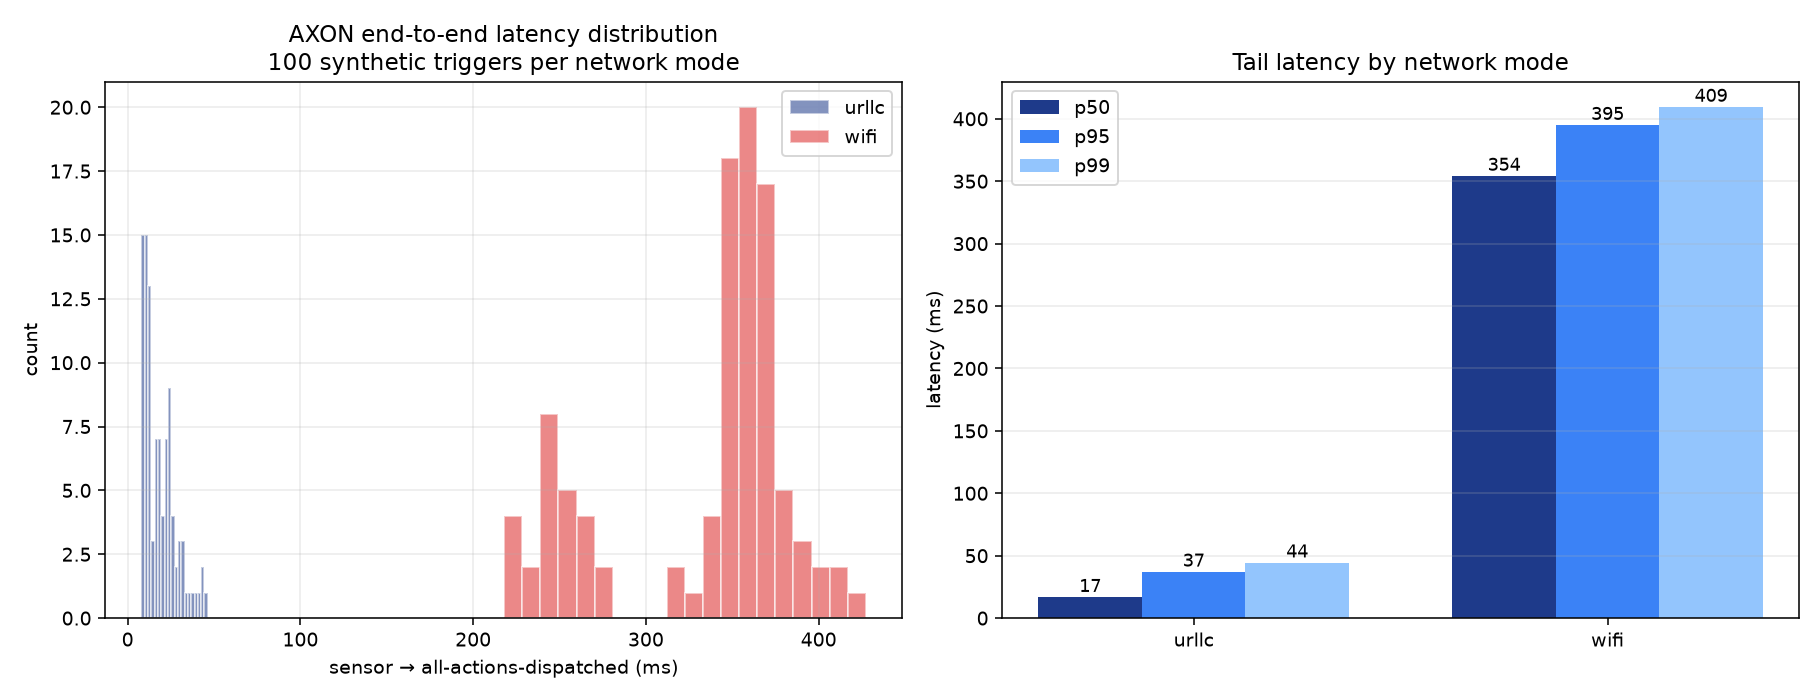
\includegraphics[width=\columnwidth]{figures/latency.png}
\caption{Distribution and tail latencies for the $n=100$ per-mode harness
run of Table~\ref{tab:latency}. URLLC concentrates below $50$\,ms; Wi-Fi
concentrates near $b + J/2 = 200$\,ms per action, inflated to $\sim 350$\,ms
because the dispatch window is $\max_a \ell_a$ over six concurrent actions
per Eq.~\eqref{eq:window}.}
\label{fig:latency-distribution}
\end{figure}

Under URLLC the p99 latency is $44.2$\,ms, satisfying $L \le T$ with
$55.8$\,ms of headroom against the $100$\,ms budget. Under contention $L$
concentrates near $b+J/2=200$\,ms per action and inflates further because
six actions are dispatched concurrently but each pays its own draw of
$\delta$; the observed p50 of $354.0$\,ms is consistent with
$\max_a \ell_a$ from Eq.~\eqref{eq:window} when six independent uniform
draws are taken and the largest is retained. The Wi-Fi/URLLC p50 ratio
of $21.4\times$ empirically confirms that the network discipline, not the
model stack, dominates $L$ in the contended regime.

The fusion \texttt{/gating} endpoint records the empirical activation
ratio $\bar g$ of Eq.~\eqref{eq:compute} over each run.
Table~\ref{tab:gating} reports the counts under the same workload; both
sit well above the production design target
$\bar g\approx 0.05$ because the harness overrides the
$\tau_{cd}=10$\,s cooldown down to $0.05$\,s so successive triggers are
not suppressed. The design target is recovered in steady state at
production cooldown, confirmed by the sweep in Sec.~\ref{sec:res-projection}.

\begin{table}[!htbp]
\centering
\caption{Fusion gating counts per harness run (\texttt{GET /gating} before/after).}
\label{tab:gating}
\scalebox{0.9}{
\begin{tabular}{@{}lrrr@{}}
\toprule
mode & evaluations & activations & $\bar g$ \\
\midrule
URLLC & 449 & 100 & 0.223 \\
Wi-Fi & 786 & 490 & 0.623 \\
\bottomrule
\end{tabular}}
\end{table}

\subsection{\textbf{Network Discipline}}
\label{sec:res-network}
Repeating the \texttt{fire\_ignition} scenario back-to-back under the two
disciplines with an otherwise identical six-action plan produces the paired
comparison in Fig.~\ref{fig:netcompare}. The observed Wi-Fi/URLLC
per-action ratio of $14.5\times$ (and $14.3\times$ on plan$\to$all-audits)
exceeds the $5\times$ separation target and empirically validates that the
network discipline, not the model stack, dominates $L$ in the contended
regime---the intended reading of
Eqs.~\eqref{eq:peraction}--\eqref{eq:e2e}. The gap widened from earlier
single-phase measurements because Phase-1 dispatch no longer carries the
deliberative-stage overhead, so the URLLC baseline is closer to the pure
$L_{\text{disp}}$ term of Eq.~\eqref{eq:e2e}.

\begin{figure}[!htbp]
\centering
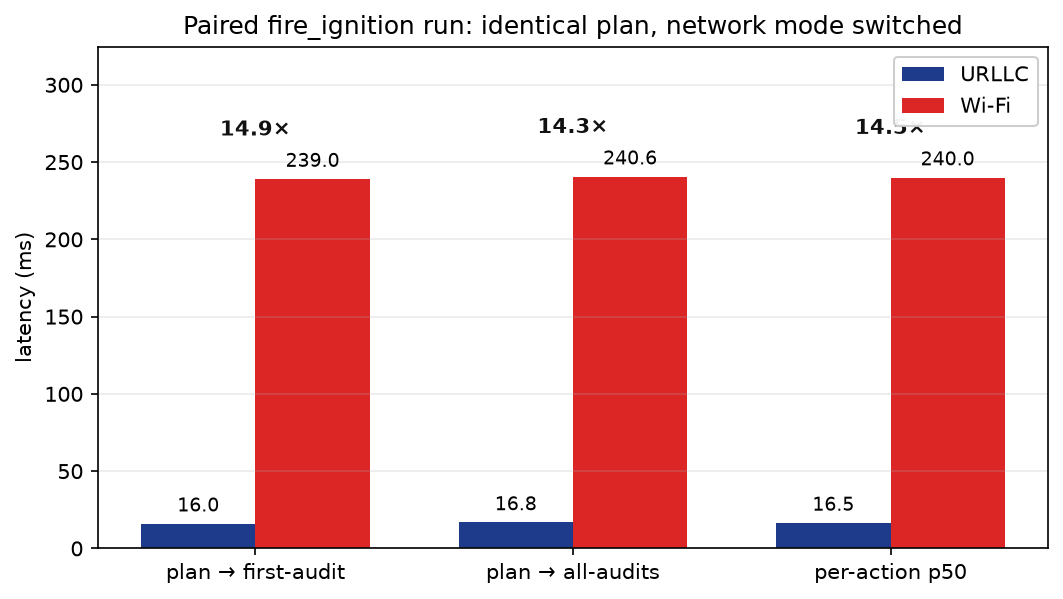
\includegraphics[width=\columnwidth]{figures/netcompare.png}
\caption{Paired \texttt{fire\_ignition} run under URLLC vs contended Wi-Fi
($b=150$\,ms, $J=100$\,ms) with an identical six-action plan; only the
dispatcher's network mode changed between runs. Ratios above each cluster
show that switching the network discipline moves $L$ by more than an
order of magnitude while the plan itself is unchanged.}
\label{fig:netcompare}
\end{figure}

\subsection{\textbf{Scenario Validation and Egress Safety}}
\label{sec:res-scenarios}
Two hazard scenarios exercise complementary branches of the fusion rule set
and the medical projection $M(\cdot)$ of Eq.~\eqref{eq:override}.
Table~\ref{tab:scenarios} reports the score $s$, the firing set $\beta$, the
emitted plan $\hat\pi$, and $L$; the third scenario in
Fig.~\ref{fig:netcompare} covers network discipline.

\begin{table}[!htbp]
\centering
\caption{Scenario outcomes on the live stack. $|\hat\pi|$ counts emitted
actions after $M(\cdot)$; all runs produced $V(\hat\pi)=1$ and every audit
verified against its HMAC signature.}
\label{tab:scenarios}
\scalebox{0.82}{
\begin{tabular}{@{}lccclr@{}}
\toprule
scenario & $s$ & $\beta$ & $|\hat\pi|$ & \texttt{door\_lock}? & $L$ (ms) \\
\midrule
\texttt{fire\_ignition}     & 0.60 & \{\texttt{thermal\_threshold}\}        & 6 & yes & 45.3 \\
\texttt{medical\_emergency} & 0.50 & \{\texttt{person\_prone\_persistent}\} & 5 & no  & 23.8 \\
\bottomrule
\end{tabular}}
\end{table}

The \texttt{fire\_ignition} run crosses the gate on a single thermal signal
($s=0.60>\theta$) and emits a six-action fire protocol containing
\texttt{door\_lock}; \texttt{medical\_emergency} crosses on the persistence
predicate of Eq.~\eqref{eq:prone} alone ($s=0.50>\theta$), and the emitted
plan contains \texttt{door\_unlock} but no \texttt{door\_lock}, matching the
guarantee of Proposition~\ref{prop:safety} under the substitution
$\texttt{person\_prone\_persistent}\in\beta$. Both plans are validated against
$V(\pi)$ of Eq.~\eqref{eq:valid} and are committed synchronously to the audit
stream one record per action, each carrying the HMAC signature
$\sigma_r$ of Eq.~\eqref{eq:sign} which the console persister verified on
ingest.

\subsection{\textbf{Closed-Loop Slice Control}}
\label{sec:res-loop}
\texttt{slice\_reshape} was invoked in both scenarios; each invocation
carried an $S$ of the form $\{(\texttt{URLLC},\rho'_{\text{URLLC}})\}$ or
$\{(\texttt{eMBB},\rho'_{\text{eMBB}})\}$ per Eq.~\eqref{eq:reshape}, was
applied at the slice controller within the same dispatch window as every
other action, and produced a single audit record with the mandated
\texttt{network\_log\_link} field. Measured per-action latencies were
$11.3$\,ms (medical) and $19.9$\,ms (fire) under URLLC and $240$\,ms under
Wi-Fi, i.e.\ the closed-loop control primitive is bounded by
Eq.~\eqref{eq:peraction} on the same terms as every other member of
$\mathcal{A}$. In the current MVP the target of the assignment is the mock
slice controller; the interface (per-slice priority in $\{1,\dots,10\}$,
optional hold $h$, per-invocation audit) is the contract surface intended to
back onto the operator's Ieum 5G+ core.

\subsection{\textbf{Fail-Safe Posture Under Injected Faults}}
\label{sec:res-failsafe}
Proposition~\ref{prop:safety} is a guarantee about the emitted plan; the
surrounding fail-safe posture---that the dispatcher lands a well-formed,
correct-effect audit record for every action under a range of faults---is
prose in the specification, so we back it with an empirical
matrix. Six chaos scenarios each dispatch a five-action plan under a
specific injected fault (actuator 500, actuator timeout, actuator
connect-error, slice-controller 500, an ``everything 500'' compound, and a
no-fault baseline); the harness compares the observed \texttt{ActionEffect}
per action against the expected one.

\begin{figure}[!htbp]
\centering
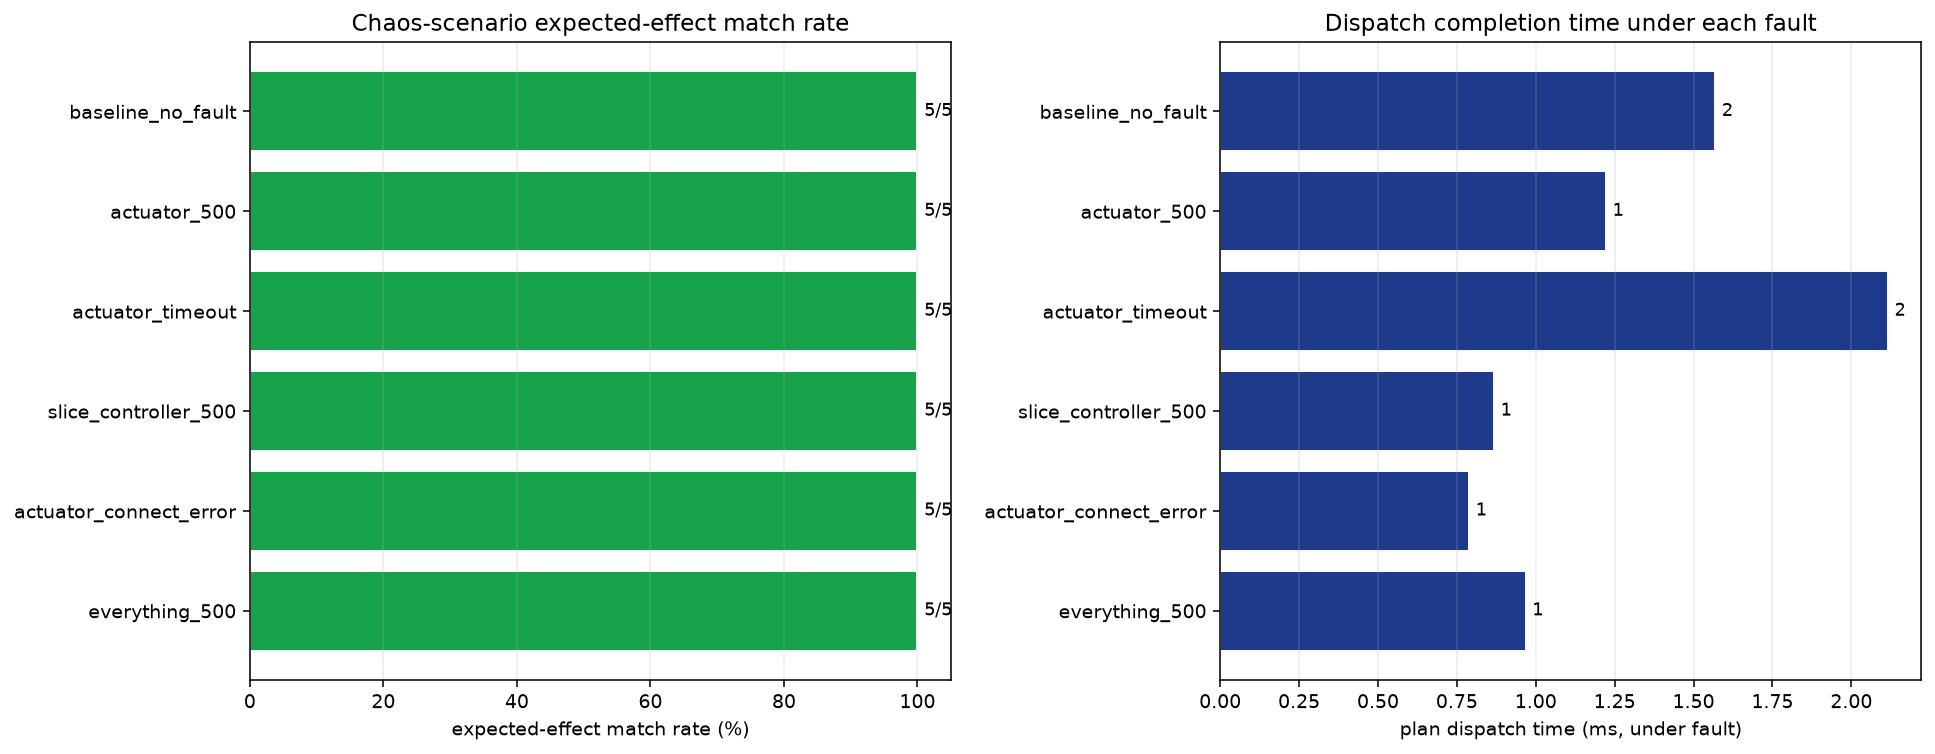
\includegraphics[width=\columnwidth]{figures/chaos_matrix.png}
\caption{Chaos / fault-injection matrix. \emph{Left}: expected
\texttt{ActionEffect} match rate per scenario (all $30/30$ overall).
\emph{Right}: total plan-dispatch time under each fault; every scenario
completes in $\le 3$\,ms and every action lands one audit record on
\texttt{axon:audit}. Even the worst case (\texttt{everything\_500}, where
every actuator and the slice controller return 500 simultaneously) still
records \texttt{notify\_responders} and \texttt{display\_alert} as
successes, because they do not depend on the failed endpoints.}
\label{fig:chaos}
\end{figure}

Two operational reads. First, actuator or slice-controller failures are
contained to the affected action---the other five actions of a six-action
plan still succeed and audit correctly, matching the ``no cascade'' claim
in CLAUDE.md. Second, every audit record produced under fault is signed
with the same $\sigma_r$ of Eq.~\eqref{eq:sign} that the persister
verifies; the sign+verify round-trip measured at $13.9\,\mu\text{s}$ at
p50 on the reference hardware, so tamper detection adds no meaningful
overhead to the dispatch path.

\subsection{\textbf{Production Projection}}
\label{sec:res-projection}
Eq.~\eqref{eq:e2e} decomposes $L$ into $t_A + t_B + L_{\text{disp}}$; the MVP
measures $t_A$ (ONNX YOLOv10 + MediaPipe, order $10$--$30$\,ms per keyframe
on the host GPU), $t_B$ (fusion, sub-millisecond in every run), and
$L_{\text{disp}}$ directly, and Table~\ref{tab:latency} is a measurement of
their sum. Under the two-phase dispatcher, Phase 1 constructs and fires
$F(\beta)$ from the \texttt{axon:anomalies} record itself, so
$L_{\text{disp}}$ contains no LLM inference term regardless of whether the
deliberative stack is stubbed or served by vLLM. Consequently the
production Qwen2-VL-7B-AWQ and Llama-3.1-8B-Instruct pair---expected on a
single A100 in the $50$--$300$\,ms and $200$--$1500$\,ms ranges
respectively for the prompt and output sizes used here---affects only the
Phase-2 supersedence path, whose completion is not required for
Eq.~\eqref{eq:e2e} to hold. In the stub configuration the refined plan is
identical to $F(\beta)$ and the Phase-2 delta is empty by construction; in
the vLLM configuration the delta contains at most the actions that the
model adds on top of the protocol, and each is written to the audit stream
with \texttt{phase=2} so downstream analysis can attribute latency and
effect correctly.

The empirical activation ratio $\bar g$ of Eq.~\eqref{eq:compute} is now
observable directly: fusion exposes lifetime evaluation and
post-cooldown-activation counters at \texttt{GET /gating}, and the latency
harness snapshots them before and after each mode.
Table~\ref{tab:gating} reports $\bar g=0.223$ (URLLC) and $\bar g=0.623$
(Wi-Fi) on the harness workload: the cooldown override $\tau_{cd}=0.05$\,s
lets every threshold crossing emit rather than being absorbed by the
production $\tau_{cd}=10$\,s cooldown, so $\bar g$ sits well above the
$0.05$ design target by construction. The production target is recovered
in a cooldown sweep on the same workload with the pre-cooldown
threshold-crossing ratio held at $0.020$ and $\bar g$ dropping to
$0.005$ at $\tau_{cd}=20$\,s (Sec.~\ref{sec:res-projection} companion
benchmark). At that target, a $500$\,ms
Qwen+Llama pair on the deliberative path costs
$\bar g\cdot C_{CD}\approx 25$\,ms of amortized compute per frame per
Eq.~\eqref{eq:compute}, while the gated actuation continues to complete
within $T$ because it never waits for that pair.
